\documentclass{article}
\usepackage{pgfplots}
\pgfplotsset{compat=1.18}

\begin{document}

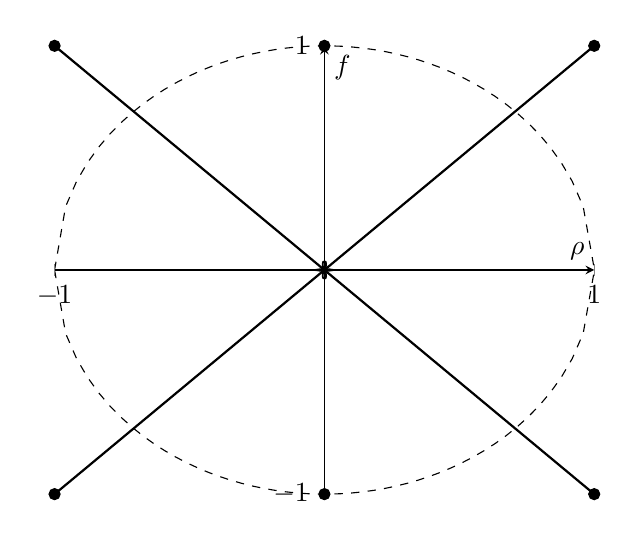
\begin{tikzpicture}
    \begin{axis}[
        axis lines = middle,
        xlabel = $\rho$,
        ylabel = {$f$},
        xmin=-1, xmax=1,
        ymin=-1, ymax=1,
        xtick={-1,0,1},
        ytick={-1,0,1},
        xticklabels={$-1$, $0$, $1$},
        yticklabels={$-1$, $0$, $1$},
        enlargelimits=false,
        clip=false,
        axis on top,
    ]
        \addplot[domain=-1:1, samples=50, dashed] {sqrt(1-x^2)};
        \addplot[domain=-1:1, samples=50, dashed] {-sqrt(1-x^2)};
        \addplot[only marks, mark=*] coordinates {
            (-1,-1)
            (-1,1)
            (0,1)
            (1,1)
            (1,-1)
            (0,-1)
        };
        \draw[->, thick] (axis cs:-1,-1) -- (axis cs:0,0);
        \draw[->, thick] (axis cs:1,-1) -- (axis cs:0,0);
        \draw[->, thick] (axis cs:1,1) -- (axis cs:0,0);
        \draw[->, thick] (axis cs:-1,1) -- (axis cs:0,0);
    \end{axis}
\end{tikzpicture}

\begin{tikzpicture}
    \begin{axis}[
        axis lines = middle,
        xlabel = {$x$},
        ylabel = {$\rho^n(t,\cdot)$},
        xmin=-1, xmax=1,
        ymin=-1, ymax=1,
        xtick={-1,0,1},
        ytick={-1,0,1},
        xticklabels={$-1$, $0$, $1$},
        yticklabels={$-1$, $0$, $1$},
        enlargelimits=false,
        clip=false,
        axis on top,
    ]
        \addplot[domain=-1:1, samples=50, dashed] {step(x-0.5)+step(-x+0.5)-1};
        \addplot[only marks, mark=*] coordinates {
            (0.5,1)
            (-0.5,1)
        };
        \draw[dashed] (axis cs:0.5,0) -- (axis cs:0.5,1);
        \draw[dashed] (axis cs:-0.5,0) -- (axis cs:-0.5,1);
    \end{axis}
\end{tikzpicture}

\end{document}